\chapter{Coupling the Majorana Zero Mode to a Double Quantum Dot \label{chap:Results} }
%--------------------------------------------------------------------------
\begin{figure}[hbt]
    \centering
    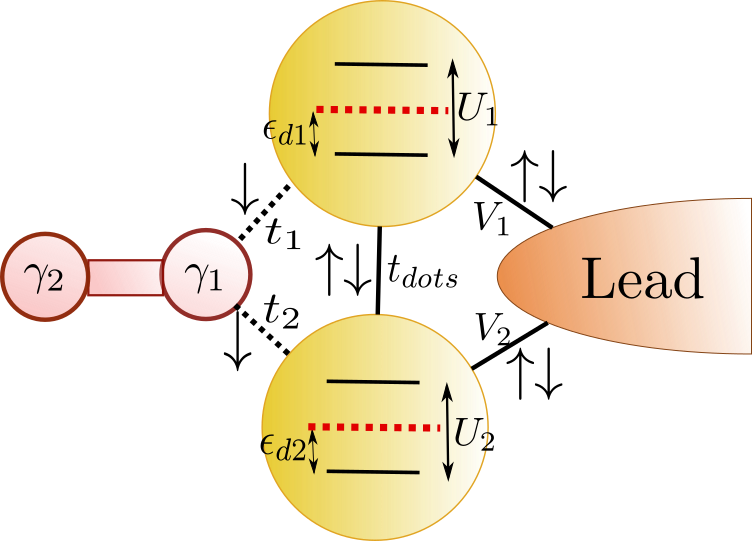
\includegraphics[scale=0.4]{IMAGES/GenModel.png}
    \caption{\label{fig:GeneralModel} General model.\\ \protect \Source{ By the Author}} 
\end{figure}


\noindent The idea of using Majorana islands formed by QDs coupled to topological superconducting wires has recently turned on new lights  into the fabrication of of quantum architectures \cite{barkeshli_physical_2015,karzig_scalable_2017}. The main insight  of this method is that today’s precise experimental control over the parameters of QDs -energy levels, tunneling couplings, etc.- offers the unique possibility of manipulating the Majorana modes inside multi-dot systems. The simplest case where Majorana manipulation is possible is in a double quantum dot. So far, no complete analysis of this basis case has been done. The purpose of this chapter is to fill this gap by realizing a full quantum transport study of the effects of coupling a Majorana mode with a double quantum dot. For this, we combine the ballistic transport and the NRG approach developed in \ref{chap: Methods}. 


% As previously stated in the , Majorana-QD  architectures turn on new lights to the area of topological quantum computing. 



% Using the ideas from the previous chapters we are going to test if it is possible to manipulate the Majorana zero mode in the double quantum dot.  

% In the previous chapter we observed the result of coupling a Majorana mode to a quantum dot. The Majorana signature characterized by a decay of the Fermi peak to the half of its original height is a



 We consider the model in \ref{fig:GeneralModel} which can be obtained from the combination of Hamiltonians of a QD-Majorana \eqref{eq:QD-Mham} and a DQD \eqref{eq:HDQD}. The Hamiltonian

\begin{equation}
H =\sum_{i=1}^2\sum_{k,\sigma}\left(\epsilon_{i}+\frac{U_i}{2}\right)d_{i\sigma}^{\dagger}d_{i\sigma}+ \frac{U_i}{2}(d_{i \sigma}^{\dagger}d_{i \sigma}-1)^{2} + t_i(\gamma d_{i,\dw}+d^\dagger_{i,\dw}\gamma) + V_id^\dagger_{i\sigma}c_{k\sigma}+V_i^* c^\dagger_{k\sigma}d_{i\sigma}.
\label{General model}
\end{equation}

% \Jesus{I neglected $\epsilon_M$ in this case. Depending on the future NRG results I will choose to add it or leave it that way. }



\section{Non-interacting case}


In order to understand the physical properties of this model, we probed a set of thought processes. The main variable in this analysis is the density of states.  We  will observe its evolution on both QDs under the tuning of the model parameters such as the majorana couplings ($t_1 , t_2$)  ,  gate voltages ($\ed{1} , \ed{2} $) and the inter dot coupling ($t_{dots}$). With these processes intend to show whether it is possible to "manipulate" the majorana modes inside the dots by tuning the established parameters. The number of possible combinations of parameters is huge and not all of them lead to important results. So on, we used the ballistic transport to select which arrangements could bring novel results. The most interesting models were simulated with NRG in the interacting case \ref{fig:Models}.  

\subsection{The Green function:}

%  To solve the transport equations using the graph method from \ref{sec:GraphMethod} first not that 
This new model is a combination the DQD graph (\ref{fig:graphDQD}) with the Majorana-QD graph \ref{fig:green-M-QD}.b). We can use the trick in \ref{sec:} to get rid of the of the Green function $\Green{f_\dw,d^\dagger_1}$ for the second Majorana operator. This allows us to obtain the following transport equations 
 
 
 
%  As we did previously in \ref{sec:GreenMaj-DQD} the transport equations for $f_\dw$ and $f^\dagger_\dw$ are 
% \begin{align}
%         \left(\omega-\epsilon_{M}\right)\Green{f_{\downarrow},d_{1\downarrow}^{\dagger}}&=\frac{t}{\sqrt{2}}\left(\Green{d_{1\downarrow},d_{1\downarrow}^{\dagger}}-\Green{d_{1\downarrow}^{\dagger},d_{1\downarrow}^{\dagger}}\right) \\
%     \left(\omega+\epsilon_{M}\right)\Green{f_{\downarrow}^{\dagger},d_{1\downarrow}^{\dagger}}&=\frac{t}{\sqrt{2}}\left(\Green{d_{1\downarrow},d_{1\downarrow}^{\dagger}}-\Green{d_{1\downarrow}^{\dagger},d_{1\downarrow}^{\dagger}}\right),
% \end{align}
% \noindent which allows us to take $\Green{f_{\downarrow}^{\dagger},d_{1\downarrow}^{\dagger}} = \frac{\omega + \epsilon}{\omega -\epsilon}\Green{f_{\downarrow}^{\dagger},d_{1\downarrow}^{\dagger}} $. Therefore, we can eliminate $\Green{f_{\downarrow}^{\dagger},d_{1\downarrow}^{\dagger}} $ from the equations even before we start Gauss-Jordan process.
 
 \begin{equation}
     \left[\begin{array}{ccccccc}
\omega-\epsilon_{1} & -V_{1}^{*} & -t_{dots} & -T_{1} & 0 & 0 & 0\\
-V_{1} & \omega-\epsilon_{k} & -V_{2} & 0 & 0 & 0 & 0\\
-t_{dots}^{*} & -V_{2}^{*} & \omega-\epsilon_{2} & -T_{2} & 0 & 0 & 0\\
-T_{1}^{*} & 0 & -T_{2}^{*} & \omega-\epsilon_{M} & -T_{2}^{*} & 0 & -T_{1}\\
0 & 0 & 0 & -T_{2} & \omega+\epsilon_{2} & V_{2}^{*} & t_{dots}^{*}\\
0 & 0 & 0 & 0 & V_{2} & \omega+\epsilon_{k} & V_{1}\\
0 & 0 & 0 & -T_{1} & t_{dots} & V_{1}^{*} & \omega+\epsilon_{1}
\end{array}\right]\left[\begin{array}{c}
\Green{d_{\mathbf{1\downarrow}},d_{1\downarrow}^{\dagger}}\\
\Green{c_{k\downarrow},d_{1\downarrow}^{\dagger}}\\
\Green{d_{2\downarrow},d_{1\downarrow}^{\dagger}}\\
\Green{f_{\downarrow},d_{1\downarrow}^{\dagger}}\\
\Green{d_{2\downarrow}^{\dagger},d_{1\downarrow}^{\dagger}}\\
\Green{c_{k\downarrow}^{\dagger},d_{1\downarrow}^{\dagger}}\\
\Green{d_{1\downarrow}^{\dagger},d_{1\downarrow}^{\dagger}}
\end{array}\right]=\left[\begin{array}{c}
0\\
0\\
0\\
0\\
0\\
0\\
1
\end{array}\right],
 \end{equation}
 
 where $T_i = \frac{t_1}{\sqrt{\omega+\epsilon_M}}$. 
 
 
% ------------------------FIGURE GRAPH--------------------
     \begin{figure}[bt]
    \centering
    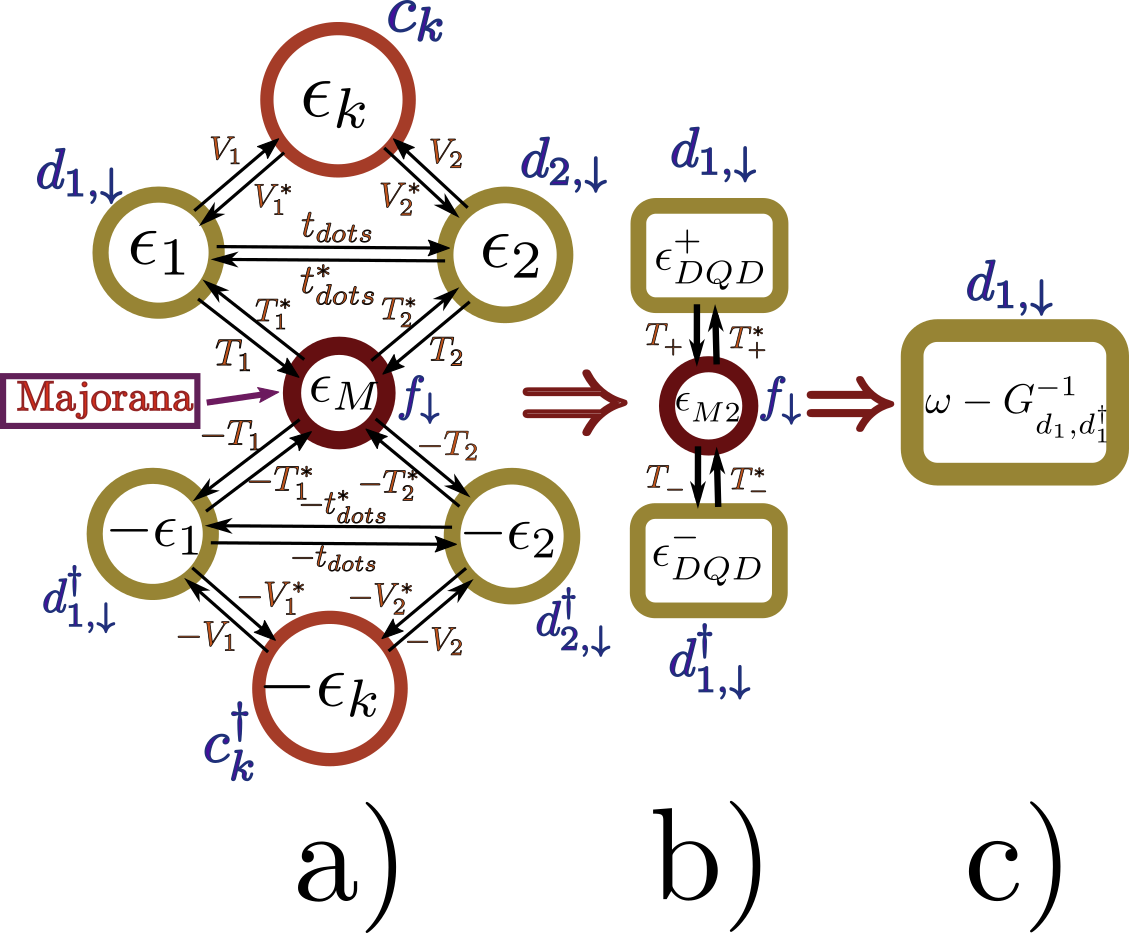
\includegraphics[scale=0.3]{IMAGES/Graphs/Final Graph.png}
    \caption{\label{fig:Graph-MDQD} Graph method applied to a DQD coupled to a Majorana zero mode. a) Initial stage. b) Popped vertexes $c^\dagger_k$, $c_k$, $d_{2, \downarrow}$ , $d^\dagger_{2, \downarrow}$ in that order. c) Popped vertexes $d^\dagger_{1, \downarrow}$ and $f_\dw$, the final energy is $\omega-\Green{d_1,d_1^\dagger}$  . \protect\Source{ By the Author  }} 
    \end{figure}

% ------------------------FIGURE GRAPH---------------------------
 The graph representing this equation is \ref{fig:Graph-MDQD}.a). Using the algorithm in \ref{sec:Algorithm} we start to popping the vertexes $c_k,c^\dagger_k, d_{2,\dw}$ and $ d^\dagger_{2,\dw}$ in that order. The energies associated to $d_{1,\dw}$ and $d^\dagger_{1,\dw}$ will be similar to the energy of the DQD \eqref{eq:EnDQD} giving 
\begin{equation}
    \epsilon_{DQD}^{\pm}=\pm\epsilon_{1}+\sum_{\mathbf{k}}\frac{V_{1}V_{1}^{*}}{\omega-\epsilon_{\mathbf{k}}}+\frac{\left\Vert \pm t_{dots}+\sum_{\mathbf{k}}\frac{V_{1}V_{2}^{*}}{\omega-\epsilon_{\mathbf{k}}}\right\Vert ^{2}}{\omega\pm\epsilon_{2}-\sum_{\mathbf{k}}\frac{V_{2}V_{2}^{*}}{\omega-\epsilon_{\mathbf{k}}}}. \label{eq:epDQD}
\end{equation}
\noindent There is also a correction in the couplings between the Majorana mode and $d_{1,\dw}$, $d^\dagger_{1,\dw}$ given by 

\begin{equation}
    T_{\pm}=\pm t_{1}\pm t_{2}\frac{\left(\pm t_{dots}+\sum_{\mathbf{k}}\frac{V_{1}V_{2}^{*}}{\omega-\epsilon_{\mathbf{k}}}\right)}{\omega\pm\epsilon_{2}\pm\sum_{\mathbf{k}}\frac{V_{2}V_{2}^{*}}{\omega-\epsilon_{\mathbf{k}}}}. \label{eq:T+-}
\end{equation}

In addition since the Majorana is in contact with dot $2$, there is an extra-term appearing in the  Majorana energy given by 
\begin{equation}
    \epsilon_{M2}=\omega-\epsilon_{M}-\frac{\frac{\omega}{\omega+\epsilon_{M}}\left\Vert t_{2}\right\Vert ^{2} } {\omega-\epsilon_{2}-\sum_{\mathbf{k}}\frac{V_{2}V_{2}^{*}}{\omega-\epsilon_{\mathbf{k}}}}-\frac{\frac{\omega}{\omega+\epsilon_{M}}\left\Vert t_{2}\right\Vert ^{2}}{\omega+\epsilon_{2}-\sum_{\mathbf{k}}\frac{V_{2}V_{2}^{*}}{\omega+\epsilon_{\mathbf{k}}}}. \label{eq:M2}
\end{equation}
It only remains to pop out vertexes $d^\dagger_1$ and $f_\dw$ in that order to obtain the green function 

\begin{equation}
    G_{{d_{1\downarrow},d_{1\downarrow}^{\dagger}}}\left(\omega\right)=\frac{1}{\omega-\epsilon_{DQD}^{+}-\frac{\left\Vert T_{+}\right\Vert ^{2}}{\omega-\epsilon_{M2}-\frac{\left\Vert T_{-}\right\Vert ^{2}}{\epsilon_{DQD}^{-}}}}.
    \label{eq:Green_NonInteracting}
\end{equation}

This simple formula summarizes the transport information through the first dot of the non-interacting Majorana-DQD system.  To compute the DOS we just need to replace once again  $\sum \frac{V_1V^*_1}{\omega -\epsilon_k}= -i\Gamma_1$ as performed in \ref{sec:GraphMethod}. By plotting the final DOS in Mathematica we were able to observe the transitions of the Majorana mode while manipulating the model parameters.  

\subsection{Theoretical results of the interacting system}
\begin{figure}[bt]
\centering
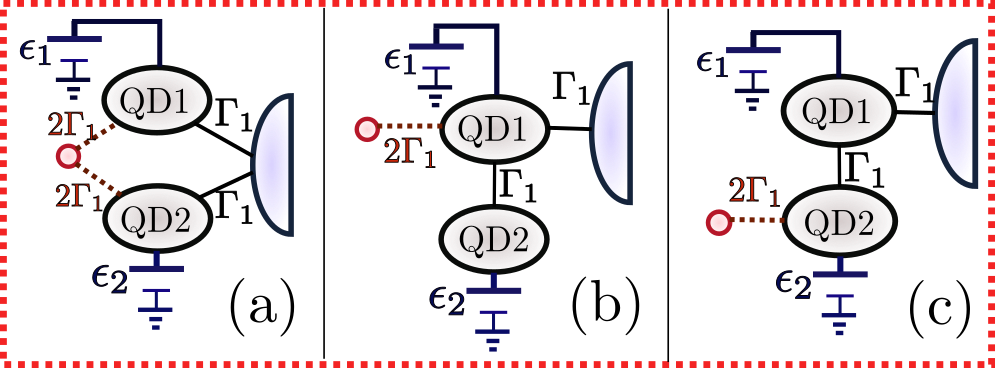
\includegraphics[scale=0.7]{IMAGES/DQD-M/3Model.png}
\caption{\label{fig:Models}. \protect\Source{By the Author}} 
\end{figure}


 %-----------F I G U R E  t1 = t2 ------
\begin{figure}[H]
    \begin{center}
    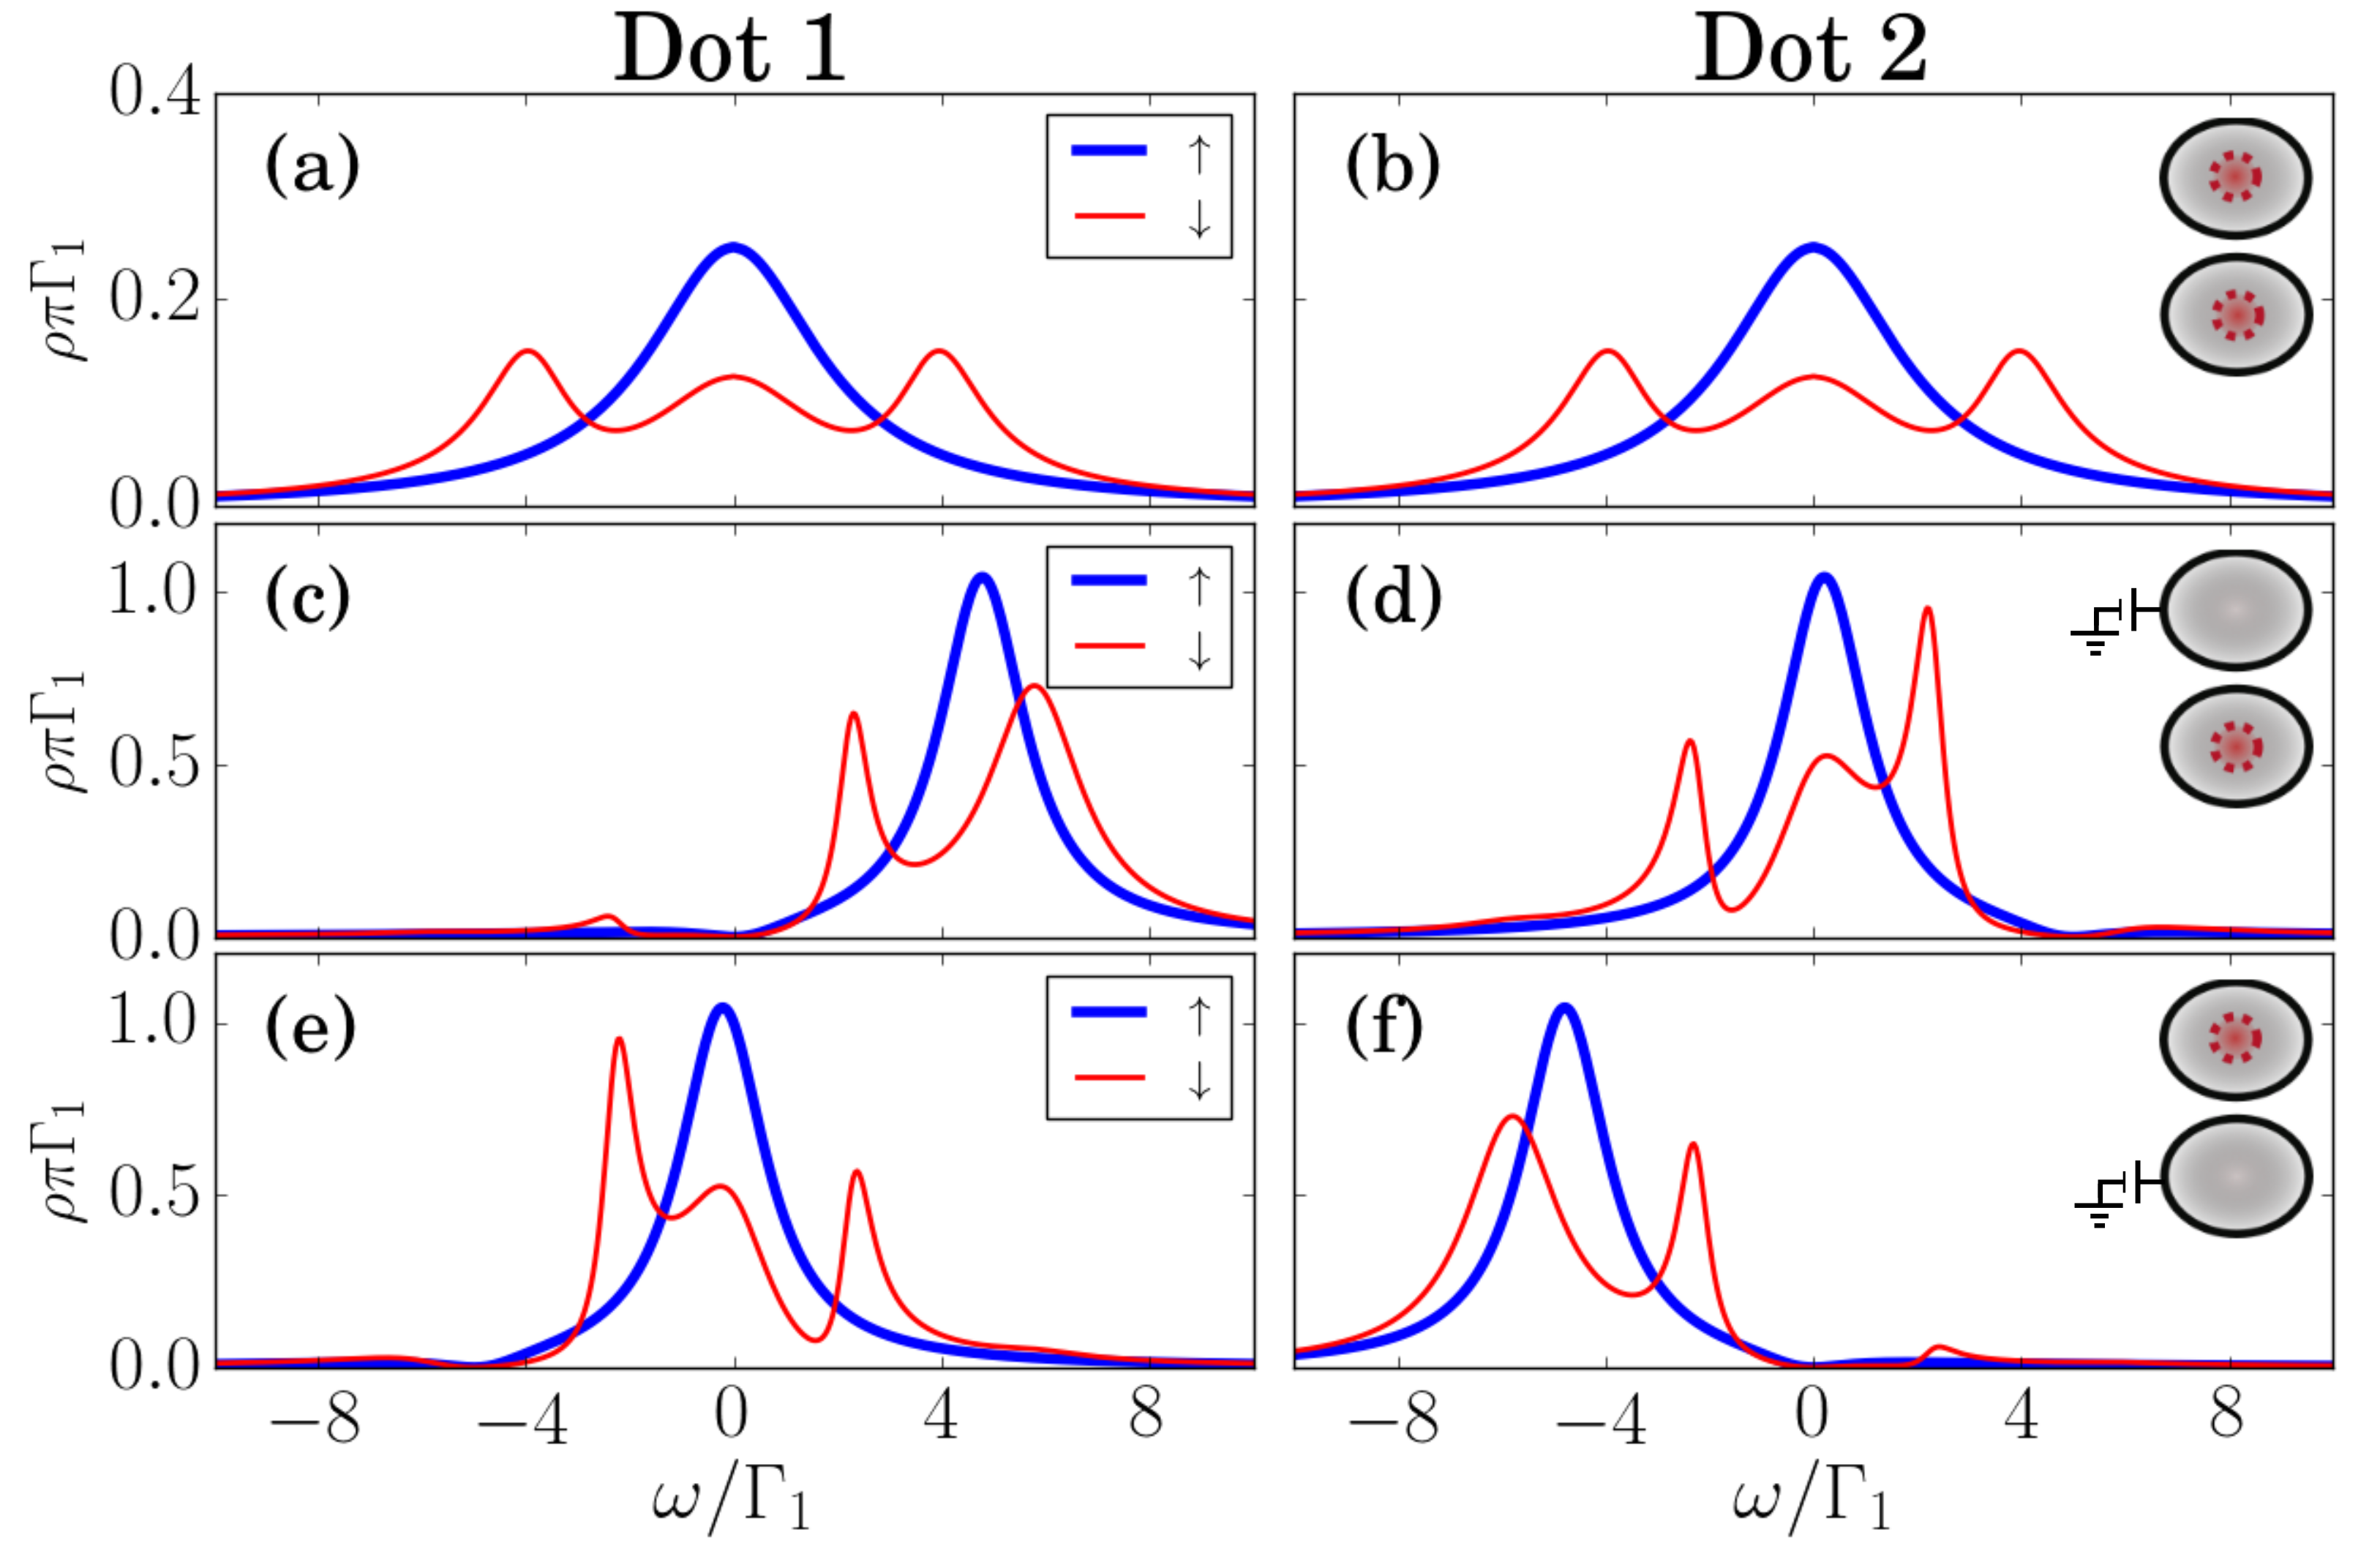
\includegraphics[scale=0.36]{IMAGES/GreenResults/t1=t2.png}
    \caption{  \label{fig:Interference} Density of states in dots 1(Left) and 2(Right) for the model \ref{fig:Models}. (a). First line (a),(b): $\ep_1=\ep_2=0$. Second line (c),(d): $\ep_1=5\Gamma_1$ , $\ep_2=0$. Third line (e),(f): $\ep_2=-5\Gamma_1$ , $\ep_1=0$.   Blue bold lines: Spin-$\up$ DOS. Red thin lines: Spin-$\dw$ DOS. The inset at the upper-right corner of each line indicates which dots  exhibit  Majorana signature, which is represented by a red dashed circle inside the dot. 
    }
    %
    \label{fig:t1=t2}
    \end{center}
\end{figure}
%-----------F I G U R E  t1 = t2 ------

In this part we will discuss the three models in figure \ref{fig:Models} which are particularly interesting for the exotic behavior of their Majorana signature. The parameters $(t_1,t_2, t_dots)$ are fixed in these three models and we will take $\ep_1$ and $\ep_2$ as variables. The first model(a), represents a symmetric coupling of the DQD with the lead and the majorana mode. In models (b) and (c) the second dot is indirectly coupled to the system through the first dot. As already analyzed in \ref{sec:GreedDQD}, the quantum interference generated by this coupling will destroy the central peak. The majorana fermion can be either connected to the first dot (b) or to the second dot (c). The system will exhibit different majorana signatures depending on which dot is connected to the Majorana zero mode.   



On each case we observe three different situations. First when there is no gate voltage $\ep_1 =\ep_2 = 0$. Second, when we turn on the first dot's gate voltage $\ep_1 = 5\Gamma_1, \ep_2 = 0$. And third, when the second dot's gate voltage is turned on $\ep_1 = 0, \ep_2 = 5\Gamma_1$. With these arrangements we expect to observe the movement of the majorana signature of each dot. 



    The manipulation of the Majorana mode is achieved by   Fig.\ref{fig:MajoranaModels} shows 9 possible processes. The first column shows a symmetric coupling of both QDs with the lead and the Majorana mode. In columns two and three the second dot is attached inderectly to the lead through the first dot. The majorana mode can be either attached to the first dot (column 2) or to the second dot (column 3). In the first row we assume that the gate voltage through both dots is $0$ $(\epsilon_1 = \epsilon_2 = 0)$, hence the density of states is particle hole symmetric $(\rho(\omega) = \rho(-\omega))$. The majorana signature can be manipulated by increasing the gate voltage at QD1 (second row) or at QD2(third row).

    The density of states for the setup in \ref{fig:Models}  (FIG.\ref{fig:MajoranaModels}) is shown in Figure \ref{fig:SymCoupling}. Since the model is non-interacting, spin-$\up$ and spin-$\dw$ models are independent. The spin-$\dw$ DOS (dashed line) shows the effects caused by the majorana mode in comparison with the spin-$\up$  results (solid line). In the particle hole symmetric case the DOS is equal in both dots. Note that that the spin-$\dw$ DOS is the half of the spin-$DOS$ at the fermi energy $\rho_\dw(0) = \rho_\up(0)$. This is a Majorana signature similar to the one observed in the single dot case \cite{liu_detecting_2011}. Hence, the majorana tunnels inside both dots. When a possitive or negative gate voltage is induced in one of the dots,  the Majorana mode is induced to leave that dot. As consequence the majorana signature will only appear in the other dot. 
     
    If the second dot is not directly connected to the lead the induced tunneling between both dots generates a path difference that destroys the central peak (See FIG\ref{fig:Interference} spin-$\up$ line). If the Majorana mode is connected to the first dot, this interference will destroy the majorana signature in the first dot. Interestingly, it is possible to observe a clear majorana signature in the second dot caracterized by a half central peak in the spin-$dw$ DOS. While turning on the first dot gate volge seems to destroy this majorana signature, tuning the second dots gate voltage returns the majorana signature to the first dot. 




 %-----------F I G U R E  t1 >0 ------
\begin{figure}[bt]
    \begin{center}
    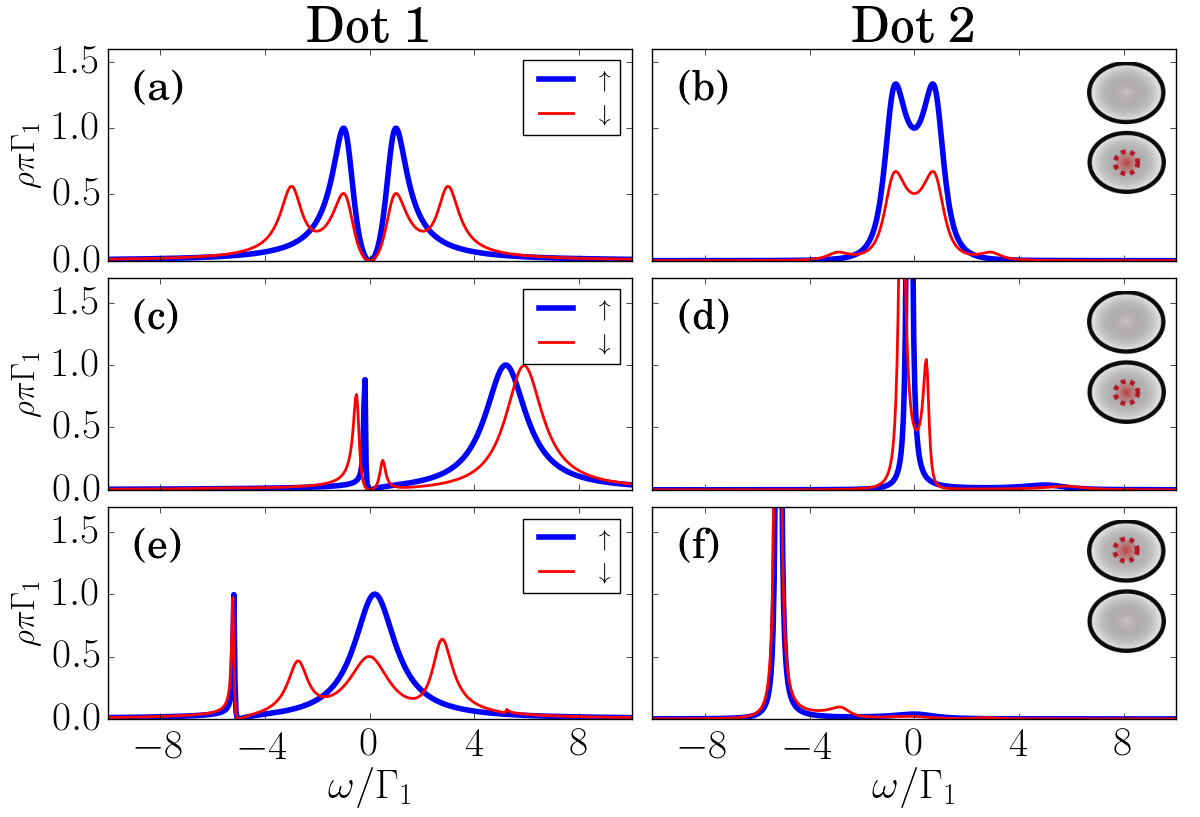
\includegraphics[scale=0.36]{IMAGES/GreenResults/t1>0,G=t2=0.png}
    \caption{  \label{fig:Interference} Density of states in dots 1(Left) and 2(Right) for the model \ref{fig:Models}. (b). First line (a),(b): $\ep_1=\ep_2=0$. Second line (c),(d): $\ep_1=5\Gamma_1$ , $\ep_2=0$. Third line (e),(f): $\ep_2=-5\Gamma_1$ , $\ep_1=0$.   Blue bold lines: Spin-$\up$ DOS. Red thin lines: Spin-$\dw$ DOS. The inset at the upper-right corner of each line indicates which dots  exhibit  Majorana signature, which is represented by a red dashed circle inside the dot. 
    }
    %
    \label{fig:t1>0}
    \end{center}
\end{figure}
%-----------F I G U R E  t1 >0 ------


 %-----------F I G U R E  t2 >0 ------
\begin{figure}[bt]
    \begin{center}
    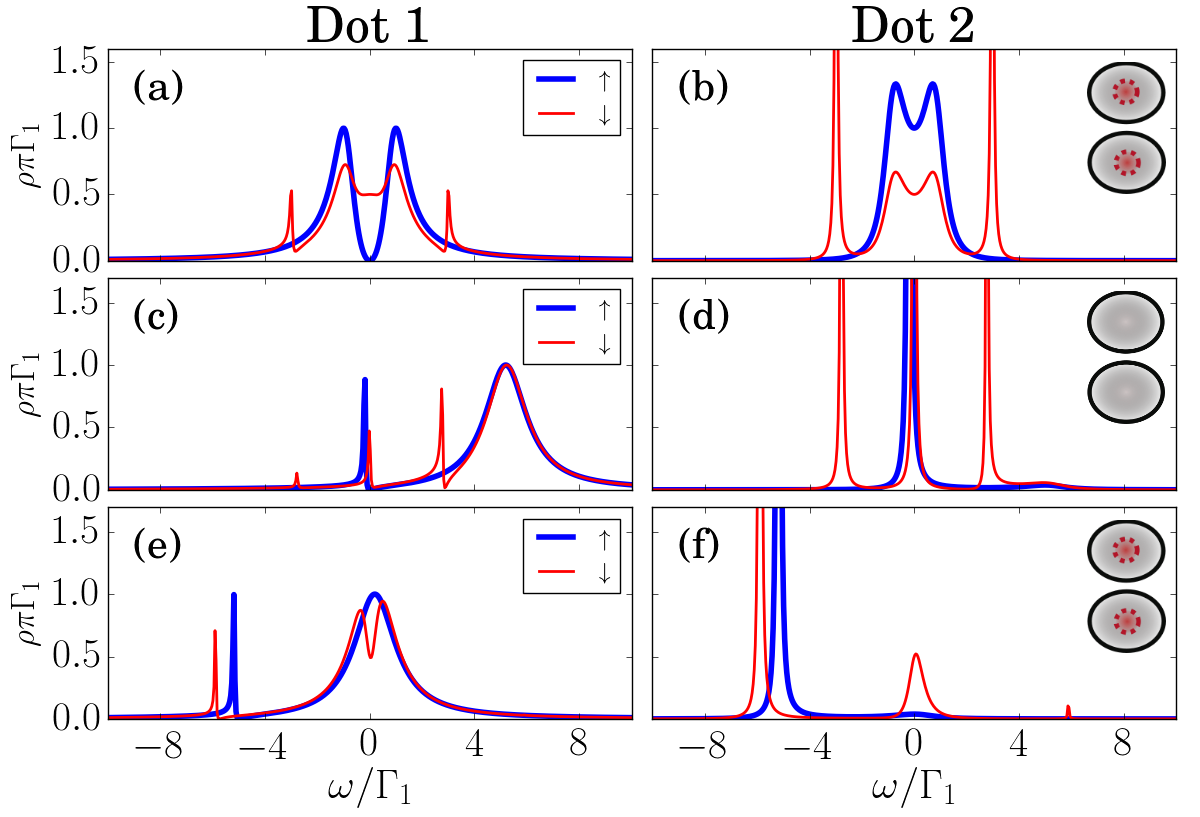
\includegraphics[scale=0.45]{IMAGES/GreenResults/t2>0,G=t1=0.png}
    \caption{  \label{fig:Interference} Density of states in dots 1(Left) and 2(Right) for the model \ref{fig:Models}. (c). First line (a),(b): $\ep_1=\ep_2=0$. Second line (c),(d): $\ep_1=5\Gamma_1$ , $\ep_2=0$. Third line (e),(f): $\ep_2=-5\Gamma_1$ , $\ep_1=0$.   Blue bold lines: Spin-$\up$ DOS. Red thin lines: Spin-$\dw$ DOS. The inset at the upper-right corner of each line indicates which dots  exhibit  Majorana signature, which is represented by a red dashed circle inside the dot. 
    }
    %
    \label{fig:t2>0}
    \end{center}
\end{figure}
%-----------F I G U R E  t2 >0 ------


 %-----------F I G U R E  4 ------
\begin{figure}[bt]
\begin{center}
\includegraphics[scale=0.48]{Graficos/t2=0.png}
\caption{  \label{fig:Interference} Density of states in both dots of the case where the only the first QD is attached to both Majorana and Lead (Fig.\ref{fig:MajoranaModels} second column) . Solid lines: Spin-$\up$ DOS. Dashed lines: Spin-$\dw$ DOS.
}
%
\label{fig:GenModel}
\end{center}
\end{figure}
%-----------E N D  F I G U R E  4 ------

 %-----------F I G U R E  4 ------
\begin{figure}[bt]
\begin{center}
\includegraphics[scale=0.48]{Graficos/t2=0.png}
\caption{  \label{fig:Interference} Density of states in both dots of the case where the only the first QD is attached to both Majorana and Lead (Fig.\ref{fig:MajoranaModels} second column) . Solid lines: Spin-$\up$ DOS. Dashed lines: Spin-$\dw$ DOS.
}
%
\label{fig:GenModel}
\end{center}
\end{figure}
%-----------E N D  F I G U R E  4 ------




\newpage


% -------------------------------------------------------------
\subsection{ a) Removing Kondo and Majorana with QD-interference \label{sec:a)}}
\Jesus{Text coming soon}

\begin{figure}[H]
    \centering
    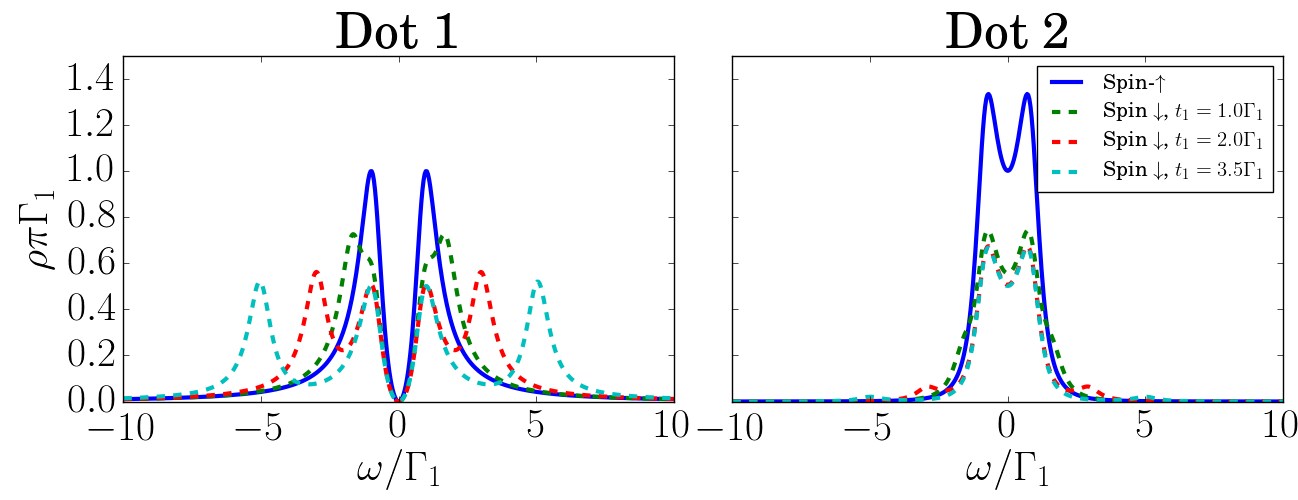
\includegraphics[scale=0.35]{IMAGES/DQD-M/a)}
    \caption{\label{fig:a)} \protect\Source{ By the Author  }}
\end{figure}

 \begin{figure}[H]
     \centering
     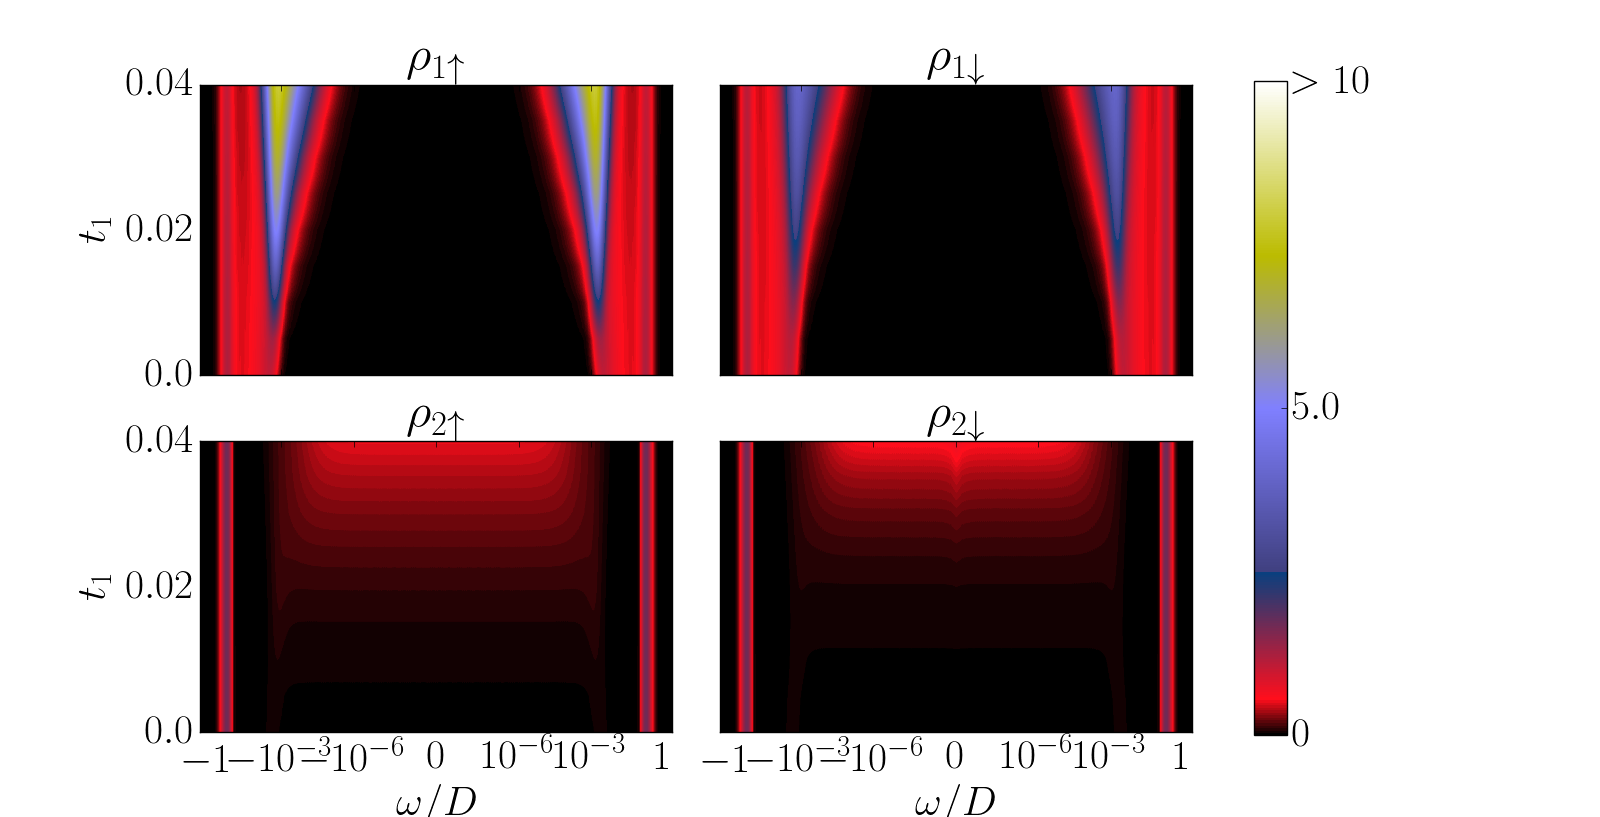
\includegraphics[scale=0.35]{IMAGES/DQD-M/a)-NRG.png}
     \caption{\label{fig:a)NRG} \protect\Source{ By the Author  } }
\end{figure}


% -------------------------------------------------------------
\subsection{ b) Indirect Majorana after Removing Kondo with QD-interference \label{sec:b)}}
\begin{figure}[H]
\centering
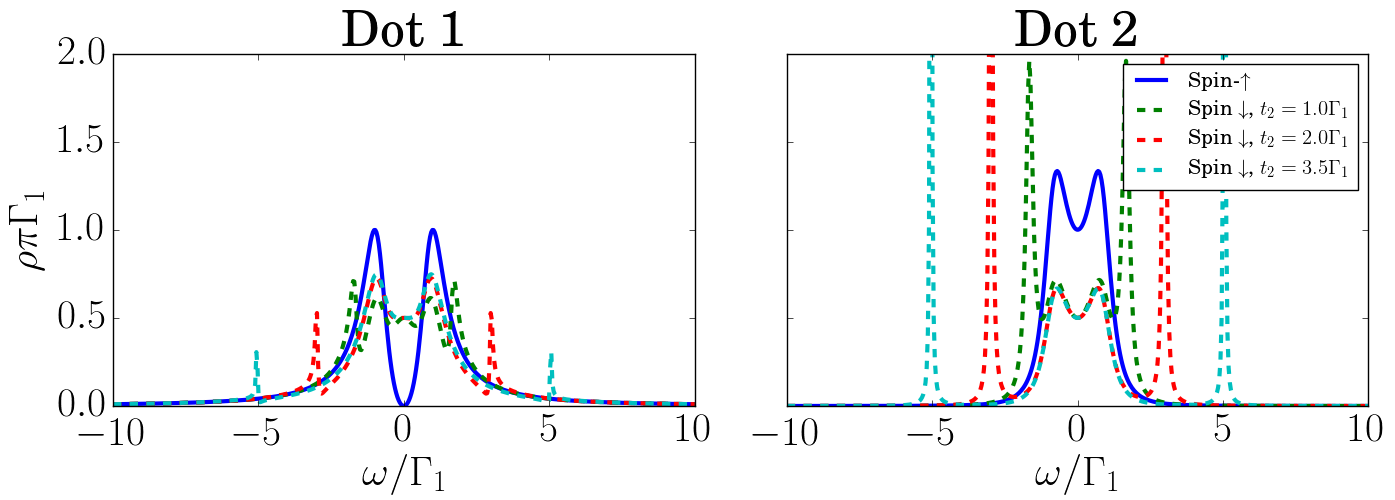
\includegraphics[scale=0.35]{IMAGES/DQD-M/b).png}
\caption{\label{fig:b)}\protect\Source{ By the Author  } }
\end{figure}

\begin{figure}[H]
    \centering
    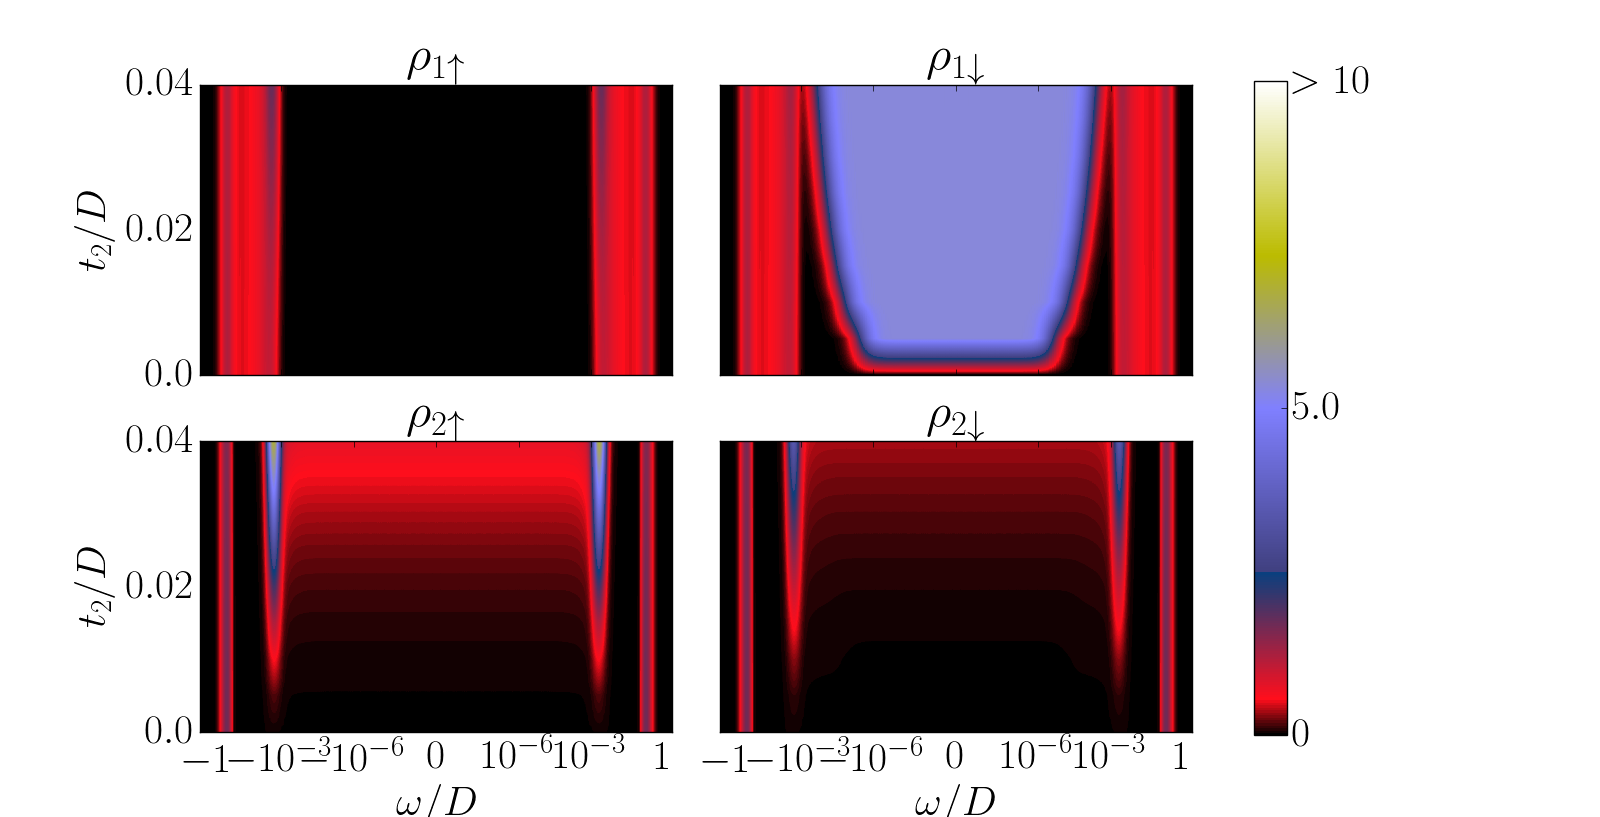
\includegraphics[scale=0.35]{IMAGES/DQD-M/b)-NRG.png}
    \caption{\label{fig:b)NRG} \protect\Source{ By the Author  }}
\end{figure}





\newpage


% -------------------------------------------------------------------
\subsection*{c) Attaching the Majorana mode to the DQD (Tuning $t_1=t_2$) \label{sec:t1=t2}}

\textbf{Parameters:}

$$\Gamma \sim 2.83*10^{-2}D, t_{dots}=0 , U_{1,2} = -2\ed{1,2} = 0.5$$
$$t_1=t_2 \in [0\  ,\  2.5*10^{-2}D]$$

\begin{figure}[hbt]
\centering
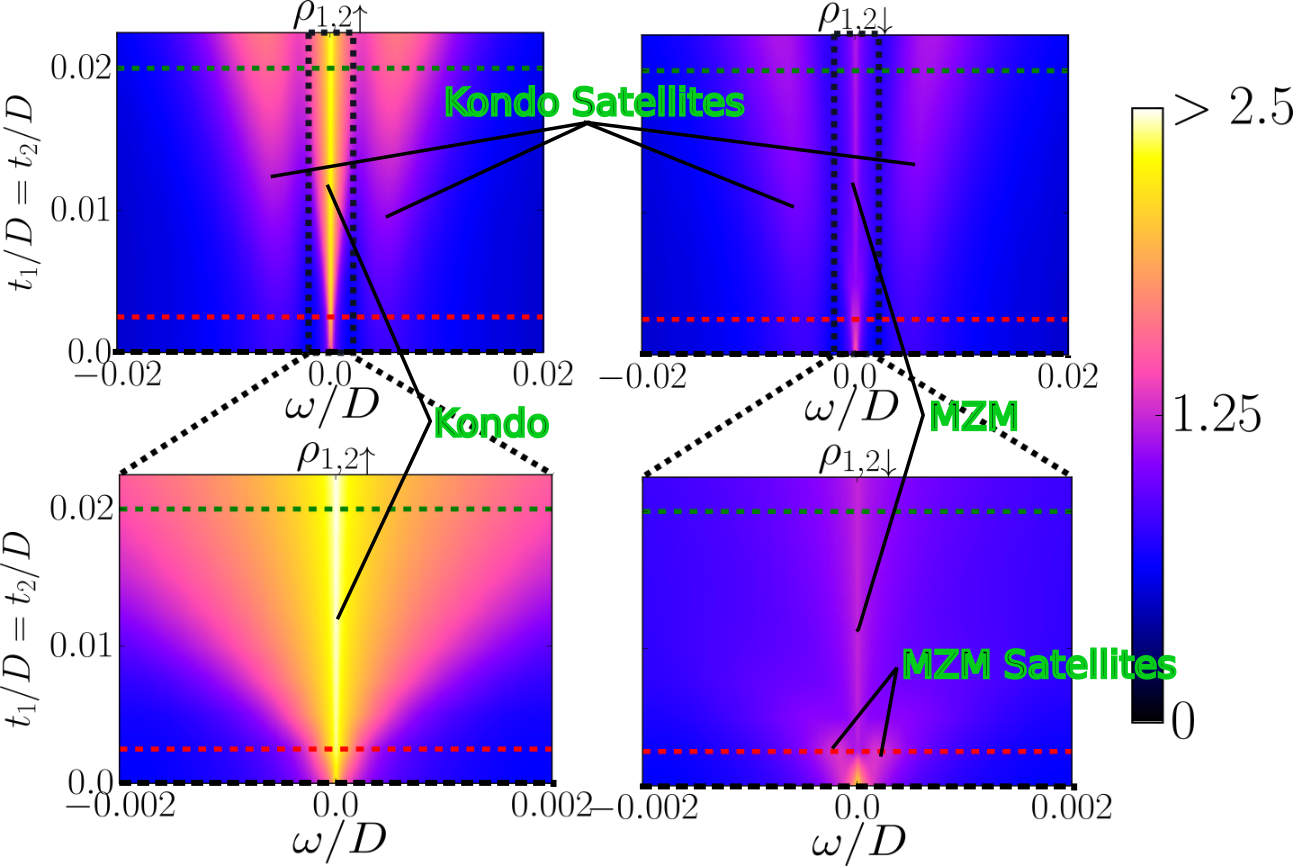
\includegraphics[scale=0.35]{IMAGES/t1=t2/2D.png}
\caption{\label{fig:2D/Shift_t1=t2} Evolution of the DOS of both QDs through $t_1 = t_2$ tuning. UP: Energy scale $\omega \sim 10^{-2}D$. DOWN: Energy scale $\omega \sim 10^{-3}D$. LEFT: Spin $\up$. RIGHT: Spin $\dw$.}
\end{figure}



The first process consists in attaching the Majorana mode to both Quantum Dots symmetrically. For this, we scale up the coupling parameter $t_1=t_2$ from $0$ (Decoupled) to $0.02$ (Completely coupled).The other parameters where chosen with an equilibrium between the dot energy and Coulomb repulsion $(\ed{1,2}=-\frac{U_{1,2}}{2})$  and  without inter-dot coupling $t_{dots}=0$. These circumstances guarantee that the system preserves Particle Hole Symmetry (PHS). Thus the Density of States (DOS) of particles and holes remains equal at all instances $(\rho(-\omega) = \rho(\omega))$. \\

\begin{figure}[hbt]
\centering
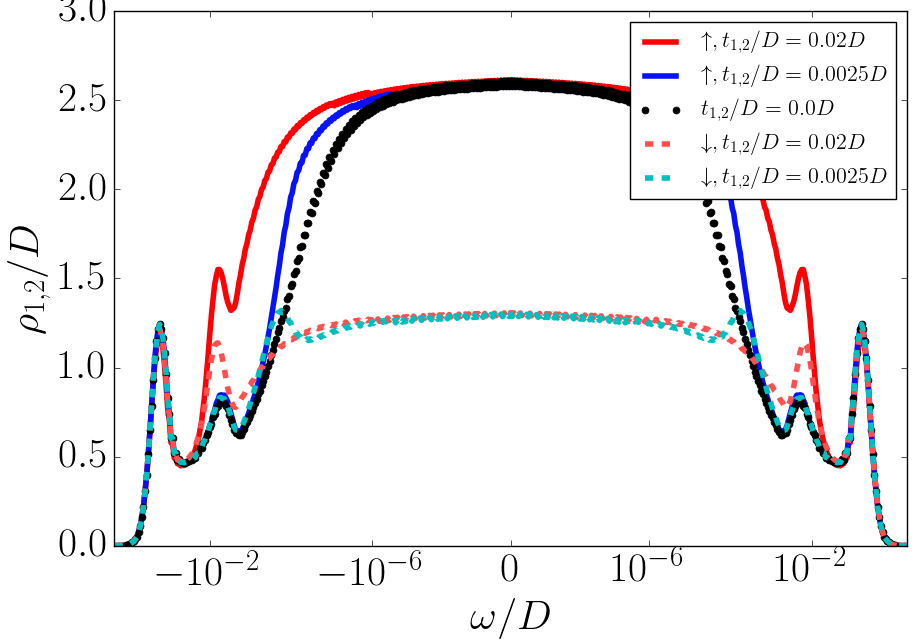
\includegraphics[scale=0.35]{IMAGES/t1=t2/LogPlot.png}
\caption{\label{fig:t1=t2/logplot} Density of states at each QD of the horizontal dashed cuts in \ref{fig:2D/Shift_t1=t2}. The energy is in logarithmic scale.  For $t_1=t_2>0$ spin-$\up$ and spin-$\dw$ DOS split near the order of $\vert \omega \vert \sim t_1,2 $. At the Fermi energy $(\omega =0)$  $\rho_\up = 2\rho_\dw$ due to the presence of the MZM in both QDs. }
\end{figure}

In the case where the majorana is detached from the DQD $(t_1 =t_2 = 0)$, the system favors the appearance of a three-peak at low energies as it is shown in \ref{fig:t1=t2/logplot} . The central peak is produced only by the Kondo effect and the two other satellite peaks are the result of a strong correlation between both dots caused by the indirect exchange of quantum states through the Lead \ref{sec:DoublePeak}. \\

Once the MZM the spin-$\up$ and spin-$\dw$ DOS split at low energies due to the new spin-$\dw$ transport channel through the Majorana mode. The spin-$\dw$ DOS at the Fermi energy ($\omega =0$) decays to the half of the spin-$\up$ DOS $\rho_\dw = \frac{\rho_\up}{2} $. By symmetry in the dot parameters this event occurs equally for both QDs. We adopt this fact as a Majorana signature. Hence we obtain that the MZM leaks inside both quantum dots. 

There is also an additional effect caused by the indirect exchange between the QDs through the Majorana mode . The consequences of this effect depend on the energy range of the majorana couplings $t_1=t_2$.  : 
\begin{enumerate}
    \item If $t_1=t_2 \ll \Gamma $ two more satellites are formed at very low energies ($\sim t_1$) in the spin-$\dw$ DOS (See  \ref{fig:2D/Shift_t1=t2} Spin-down $\omega \sim 10^{-3}D$ ). (See  \ref{fig:2D/Shift_t1=t2} Spin $\up$, $\omega \sim 10^{-3}D$ ).
    \item If $t_1=t_2 \sim \Gamma$ , the MZM contributes to the the growth of the spin-up satellites in the DOS. This effect produces the splitting between the spin-up and spin-down DOS.   (See  \ref{fig:2D/Shift_t1=t2} Spin-$\dw$, $\omega \sim 10^{-2}D$).
\end{enumerate}









% At low energies $(\omega/D \sim 10^{-2})$ \ref{fig:2D/Shift_t1=t2} shows the emergence of a 3-peak in the DOS close to the Fermi energy. This 3-peak is formed by a central peak defined by the Kondo (spin $\up$) and the Majorana (spin $\dw$) peaks. The other two peaks are generated by an indirect exchange of the states between the quantum dots through the leads (SEE ABSTRACT). At even lower energies $(\omega/D \sim 10^{-4})$ it is possible to appreciate the emergence of another 3-peak in the spin down DOS which is present only for small values of the Majorana coupling constants $t_1 = t_2 \ll 0.01D$ (See  \ref{fig:t1=t2/logplot}). These sided peaks are caused by the indirect exchange between both dots through the Majorana Mode. When the Majorana couplings achieve the same order of the dot-lead coupling $\Gamma$ $(t_1 = t_2 \sim  0.01D)$ both sided peaks are merged causing the extinction of the majorana side-peaks and the increase of the indirect exchange peaks at $(\omega/D \sim 10^{-2})$. 

% \begin{figure}[H]
% \centering
% 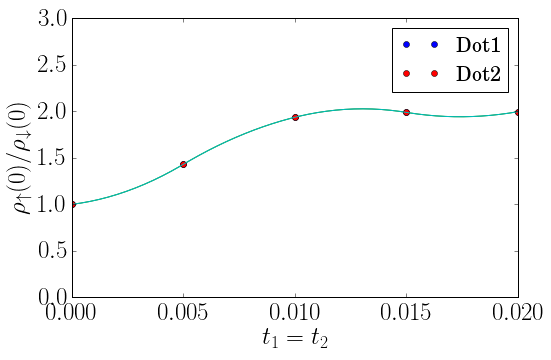
\includegraphics[scale=0.4]{Plots/MSig/Shift_t1=t2.png}
% \caption{\label{fig:MSig/Shift_t1=t2} Relation between the Zero-peaks at the fermi level. The Majorana signature is related to $\frac{\rho_\up(0)}{\rho_\up(0)}=2$.}
% \end{figure}










%--------------------------------------------------------------------

\subsection{ e) Transferring the MZM through gate voltage shifting $\ed{2}$. \label{sec:e2}}

\textbf{Parameters:}

$$\Gamma \sim 2.83*10^{-2}D, t_{dots}=0 , U_{1,2} = -2\ed{1} = 0.5 , t_1=t_2=0.0025$$
$$\ed{2} \in [-0.25 \  , -0.05]$$

This process starts with the DQD coupled symmetrically  to the Majorana mode, just as in \ref{sec:t1=t2}. The idea of this process is to break PHS by increasing the energy of the second QD $\ed{2}$. This procedure should induce the Majorana to tunnel only into the first dot. 


\begin{figure}[h]
\centering
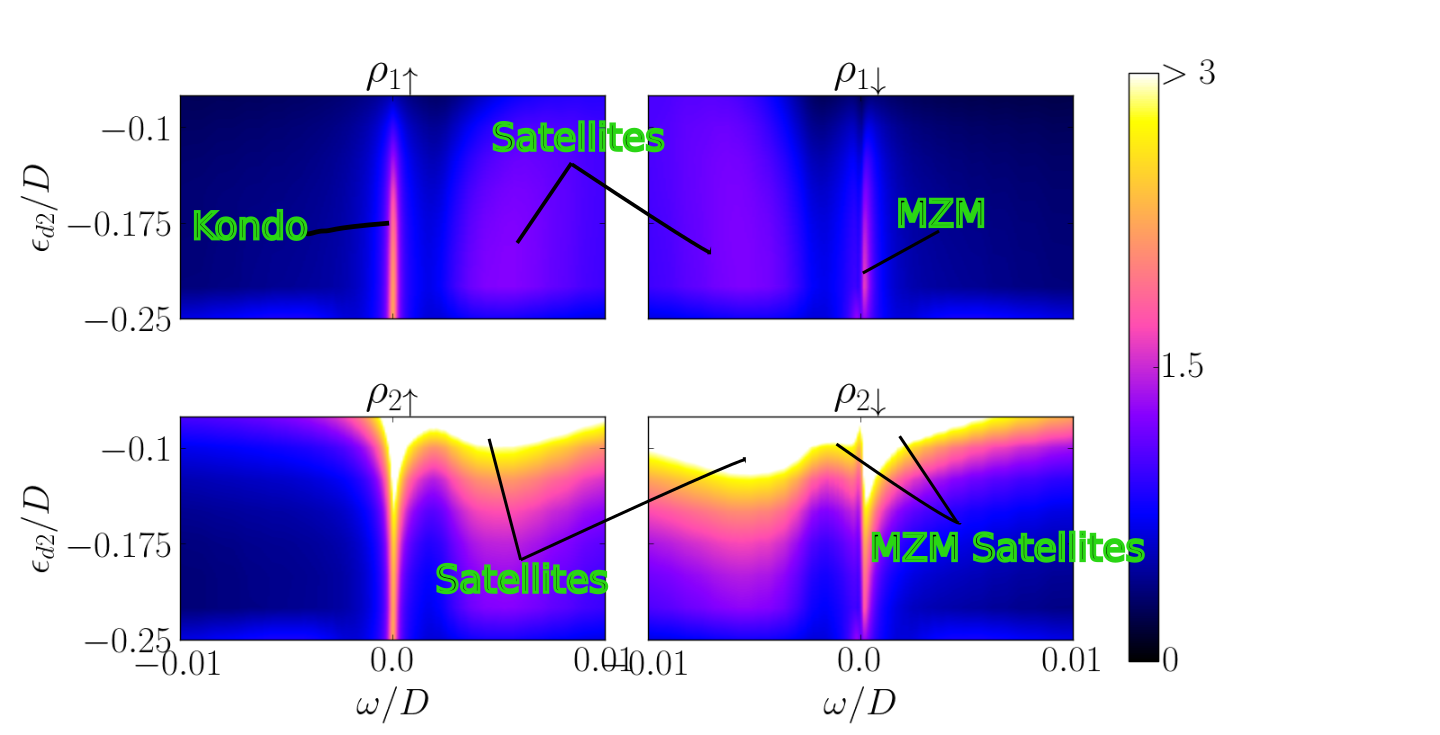
\includegraphics[scale=0.35]{IMAGES/ed2/2D.png}
\caption{\label{fig:2D/Shift_ed2} Evolution of the DOS of both QDs through the $\ed{2}$ tuning. UP: QD1. DOWN: QD2. LEFT: Spin $\up$. RIGHT: Spin $\dw$.}
\end{figure}


In \ref{fig:2D/Shift_ed2} we observe that both, the Kondo and the MZM peaks are preserved in the first QD as well as the majorana signature (See \ref{fig:ed2/Fermi}) when $\ed{2}$ is scaled up to $-0.1$.  However,  PHS breaking will favor the growth of the spin-$\up$ hole $(w>0)$  satellite and the spin-$\dw$ particle $(w<0)$ satellite.




In the second QD the DOS increases abruptly for both spins.The majorana signature is rapidly when  lost . Hence, with this set-up it is actually possible to induce the Majorana to preferably tunnel QD1 in despite of QD2.  \\
\begin{figure}[H]
\centering
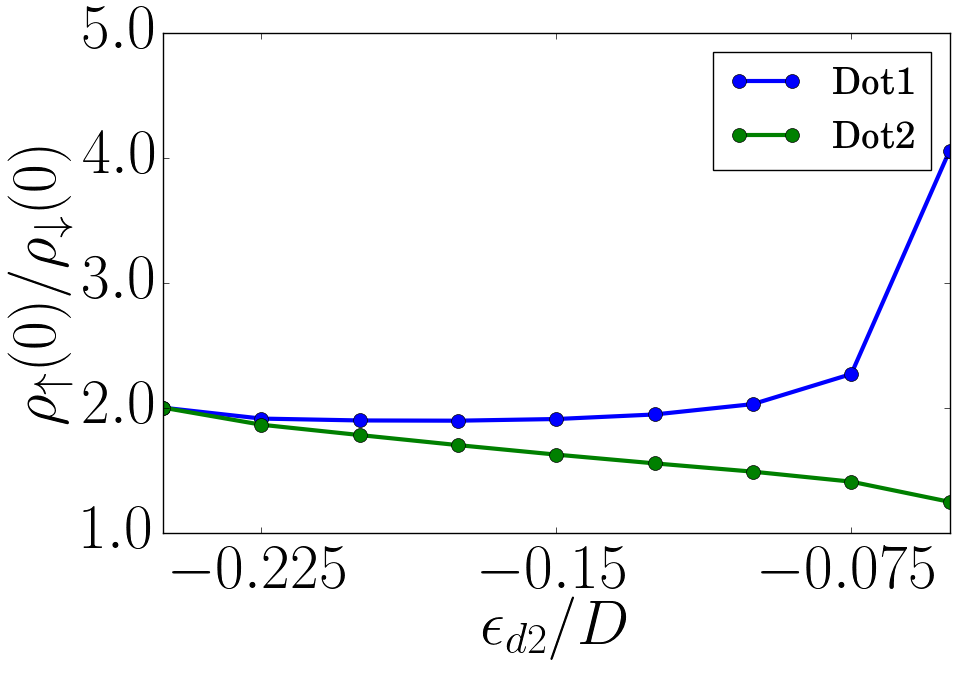
\includegraphics[scale=0.3]{IMAGES/ed2/Fermi.png}
\caption{\label{fig:ed2/Fermi} As described in \ref{sec:t1=t2} the relation $\frac{\rho_\up(0)}{\rho_\up(0)}=2$ constitutes a Majorana Signature . This picture evaluates shows the evolution of the relation $\frac{\rho_\up(0)}{\rho_\up(0)}$ for both QDs. While QD2 losses rapidly the Majorana signature, QD1 maintains it till $\ed{2}\sim -0.1$.}
\end{figure}


\newpage


%---------------------------------------------------------------------------

\section{Particle-Hole symmetric shifting of $\ed{2}=\frac{U}{2}$.}

\begin{figure*}[h]
\centering
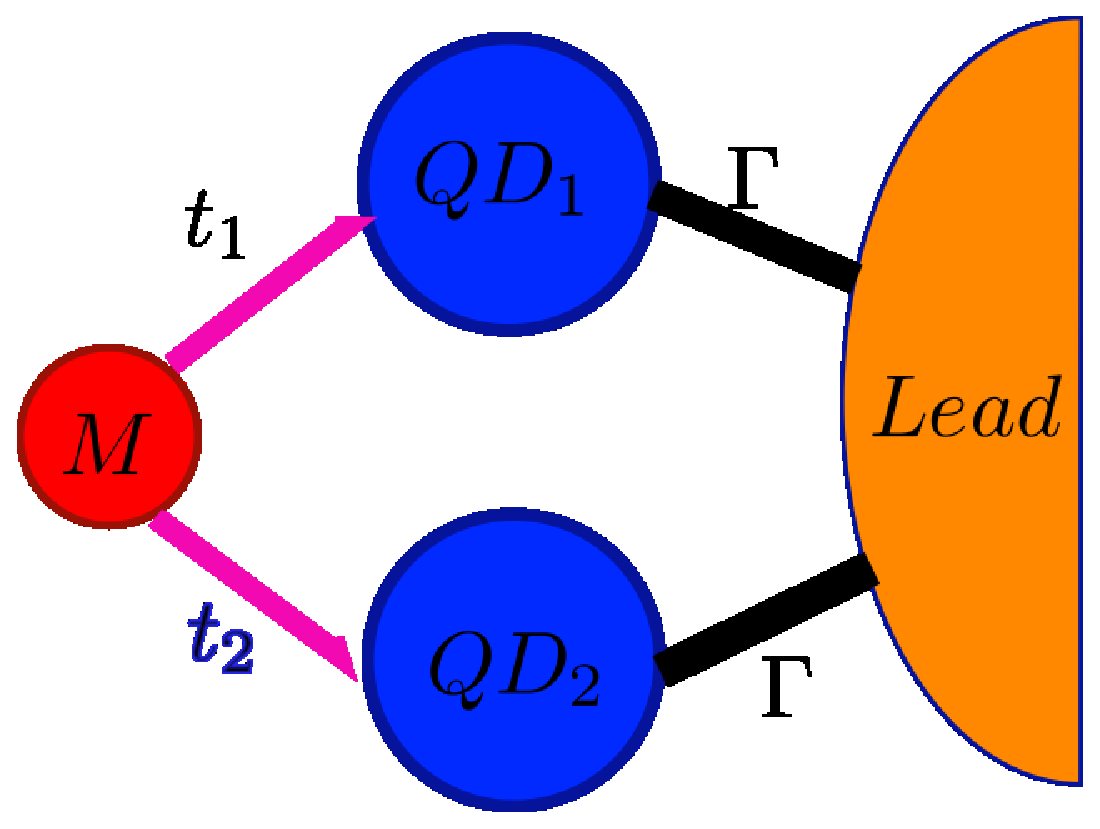
\includegraphics[scale=0.2]{Plots/Model/Majorana-2QD.eps}
\caption{\label{fig:Mod/PHS-Shift_e2.png}$U_{1}=-2\ep_{d1}=0.5$, $\Gamma_{1}=\Gamma_{2}$,
$t_{1}=t_2=0.02$. Variable $\ep_{d2} =\frac{U_{2}}{2}$}
\end{figure*}
\begin{figure}[hbt]
\centering
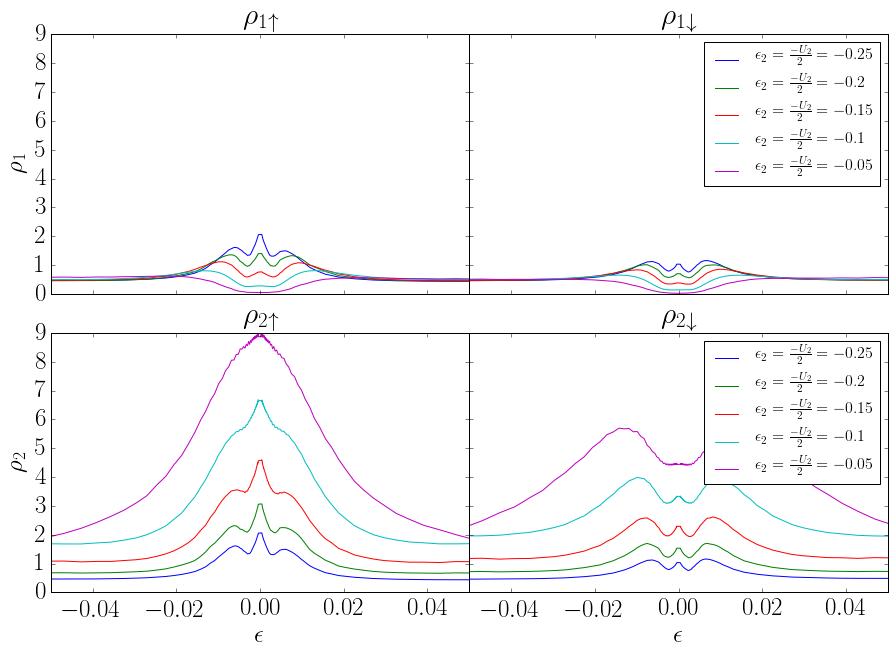
\includegraphics[scale=0.38]{Plots/DOS/PHS-Shift_e2.png}
\caption{\label{fig:DOS/PHS-Shift_e2.png} Evolution of the QDs' DOS for the model in \ref{fig:Mod/PHS-Shift_e2.png} }
\end{figure}
We start again with the symmetric model with both QDs coupled to the Majorana mode, but this time the evolution is performed over $\ep_2=\frac{U}{2}$, such that the model is always Particle-Hole symmetric. This situation is very different from the previous model (\ref{sec:e2}) since the decaying of $U2$ 
equalizes the effect of increasing the dot energy. In \ref{fig:DOS/PHS-Shift_e2.png} we observe that the DOS of QD2 increases while the QD1's DOS decreases, just as it happened in \ref{sec:e2} . However, the Majorana signature remains at $2$ for both dots , meaning that the Majorana is not preferably induced to tunnel to any QD despite the lose of symmetry in the dot energy.

% \begin{figure}[hbt]
% \centering
% 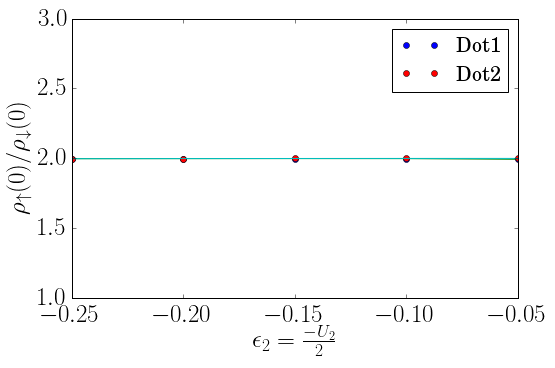
\includegraphics[scale=0.4]{Plots/MSig/PHS-Shift_e2.png}
% \caption{\label{fig:MSig/PHS-Shift_e2} Relation between the spin up-down Zero-peaks at the Fermi level. The Majorana signature is related to $\frac{\rho_\up(0)}{\rho_\up(0)}=2$.}
% \end{figure}

%---------------------------------------------------------------------------
\section{Shifting $t_2$}

%$U_{1}=U_{2}=-2\epsilon_{d1}=-2\epsilon_{d2}=0.5$, %$\Gamma_{1}=\Gamma_{2}$,
%$t_{1}=0.02$

\begin{figure*}[h]
\centering
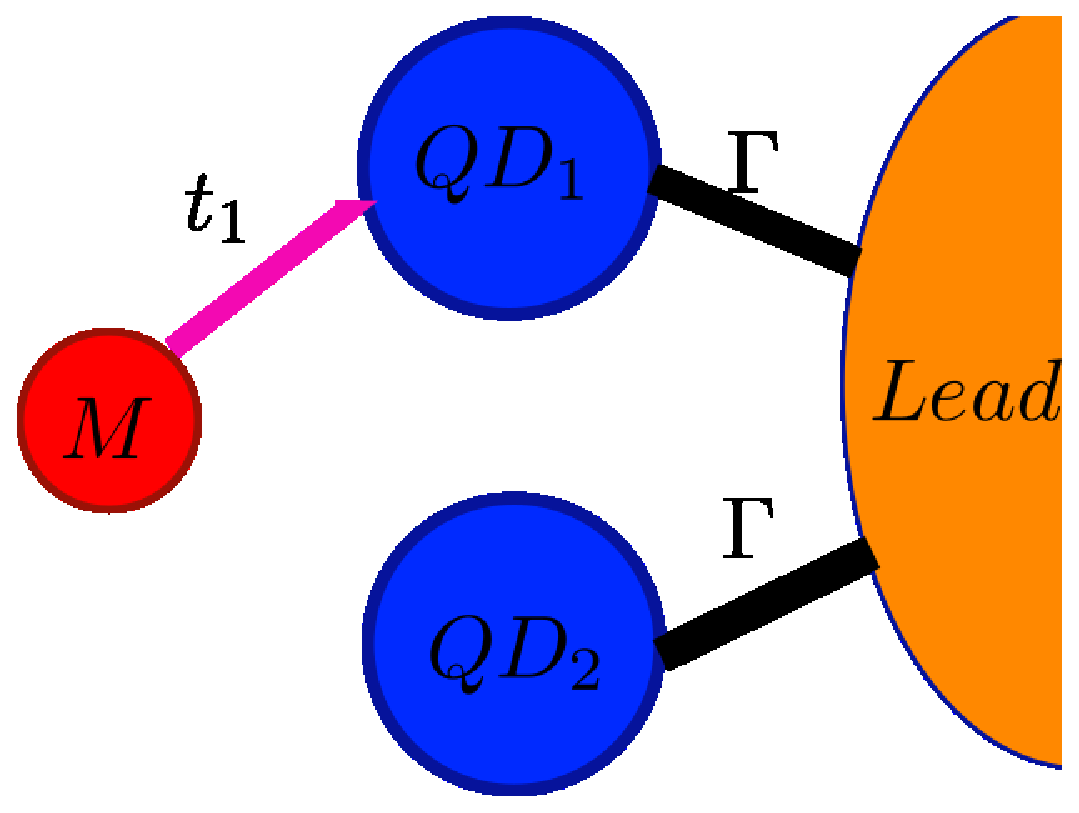
\includegraphics[scale=0.2]{Plots/Model/Majorana-1QD.eps}
\caption{\label{fig:Mod/Shift_t2}$U_{1}=U_{2}=-2\ep_{d1}=-2\epsilon_{d2}=0.5$, $\Gamma_{1}=\Gamma_{2}$,
$t_{1}=0.02$. Variable $t_2$}
\end{figure*}


\begin{figure}[hbt]
\centering
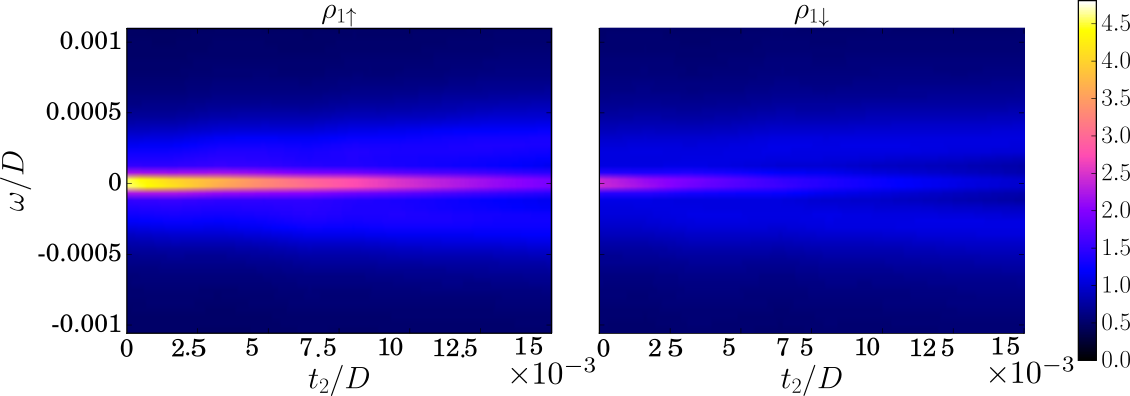
\includegraphics[scale=0.38]{Plots/2D/Shift_t2D1.png}
\caption{\label{fig:DOS/Shift_t2D1} Evolution of the DOS in the first QD }
\end{figure}
% \begin{figure}[hbt]
% \centering
% 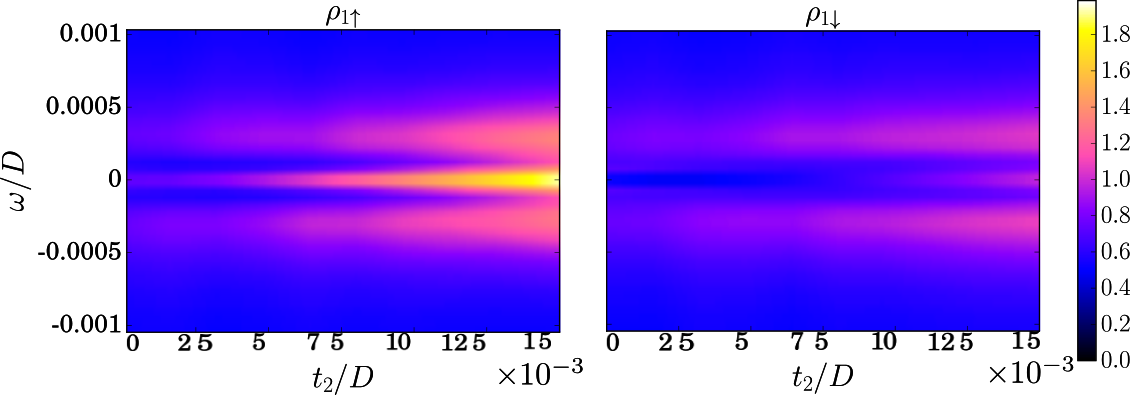
\includegraphics[scale=0.38]{Plots/2D/Shift_t2D2.png}
% \caption{\label{fig:DOS/Shift_t2D2} Evolution of the DOS in the Second QD}
% \end{figure}



\iffalse
\begin{figure}[hbt]
\centering
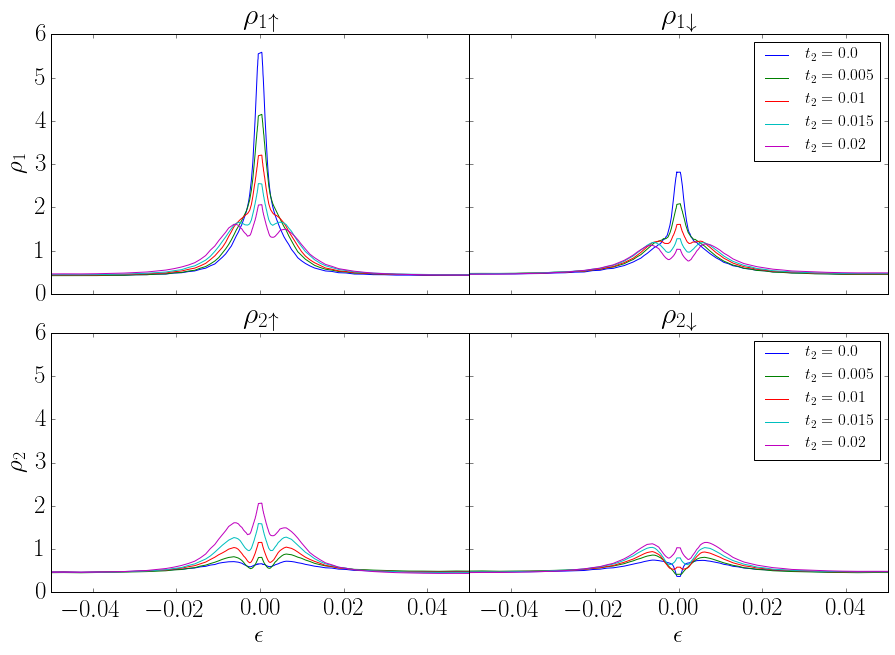
\includegraphics[scale=0.38]{Plots/DOS/Shift_t2.png}
\caption{\label{fig:DOS/Shift_t2} Evolution of the QDs' DOS for the procedure in \ref{fig:Mod/Shift_t2} }
\end{figure}
\fi
 In \ref{fig:DOS/Shift_t2D1} and \ref{fig:DOS/Shift_t2D1} we observe the evolution of DOS in the case where the second dot is smoothly connected to the Majorana, which is already attached to the first dot. The hopping parameter $t_2$ scales up to $0.015D$ where the model reaches the symmetry $t_2 = t_1$. The figures show that increasing $t_2$ leads to a drop in the DOS of QD1 while the DOS in QD2 is increased. In addition, the single peak in the first dot transforms into a three-peak due to the Majorana interference with the second dot. In \ref{fig:MSig/Shift_t2} we also observe that the reason between the zero up-down DOS  $\left(\frac{\rho_\up(0)}{\rho_\up(0)}\right)$ smoothly scales up to $2$ in QD2. At $t_2 =0.02$, when the  is completely symmetric, the Majorana signature appears in both quantum dots. Note that the relation $\frac{\rho_\up(0)}{\rho_\up(0)}$  is already close to $2$ at $t_2=0$. This implies that the second dot "feels" the Majorana even when it is not directly connected to the Majorana mode. 















% To built the ballistic transport graph (See \ref{sec:GraphMethod}) we just need to think that our model is actually merging the DQD graph (\ref{fig:graphDQD}) with the Majorana (Figure \ref{fig:green-M-QD}.b)). No need to write the green transport equations . Note  in graph $\MDQD$ that the  green function  $\Green{d_{1\downarrow},d_{1\downarrow}^{\dagger}}{\MDQD}$  is composed by the greeen function of the DQD $\left(\GreenG{d_{1\downarrow},d_{1\downarrow}^{\dagger}}{\GDQD } \right)$ and the extra term added by the presence of the majorana opperator $f_\downarrow$. In the equations this is simply 

% \begin{equation}
%     \GreenG{d_{1\downarrow},d_{1\downarrow}^{\dagger}}{\MDQD}=\left[\left(\GreenG{d_{1\downarrow},d_{1\downarrow}^{\dagger}}{\GDQD } \right)^{-1}+\frac{\omega}{\omega+\epsilon_{M}}\frac{E_{d_{1\dw}f_{\dw}}^{\MDQD}}{\left[\GreenG{f_{\downarrow},f_{\downarrow}^{\dagger}}{\MDQD-d_{1}}\right]^{-1}}\right]^{-1}.
% \end{equation}
% where 
% \begin{equation}
%     E_{d_{1\dw}f_{\dw}}^{\MDQD}=\left(t_{1}+t_{2}\frac{\left(t_{dots}+\sum_{\mathbf{k}}\frac{V_{1}V_{2}^{*}}{\omega-\epsilon_{\mathbf{k}}}\right)}{\omega-\epsilon_{2}-\sum_{\mathbf{k}}\frac{V_{2}V_{2}^{*}}{\omega-\epsilon_{\mathbf{k}}}}\right)\left(t_{1}^{*}+t_{2}^{*}\frac{\left(t_{dots}^{*}+\sum_{\mathbf{k}}\frac{V_{1}^{*}V_{2}}{\omega-\epsilon_{\mathbf{k}}}\right)}{\omega-\epsilon_{2}-\sum_{\mathbf{k}}\frac{V_{2}^{*}V_{2}}{\omega-\epsilon_{\mathbf{k}}}}\right).
% \end{equation}
% \Jesus{This fact is difficult to explain. I will need more plots and writing the appendix. For now I will leave here some results}

% We then need to compute $\GreenG{f_{\downarrow},f_{\downarrow}^{\dagger}}{\MDQD-d_{1}}$ . This graph is much simple. The neighborhood of  $f_{\downarrow}$ in graph ${\MDQD-d_{1}}$ are $d_2$ (above) and the inverted DQD(bellow). These neighbors are disconnected, hence we can include the in the green function independently. The term above is simply the dot $d_{2\downarrow}$ connected with the lead . 
% \begin{equation}
%     \frac{\frac{\omega}{\omega+\epsilon_{M}}\left\Vert t_{2}\right\Vert ^{2}}{\omega-\epsilon_{2}-\sum_{\mathbf{k}}\frac{V_{2}V_{2}^{*}}{\omega-\epsilon_{\mathbf{k}}}}.
% \end{equation}

 
% The term generated by the connection of $f_{\downarrow}$  with the inverted $DQD$ is a bit more complicated. First we need to include the term given by the connection with  $d_{2\downarrow}^\dagger$ which is 

% The other term is the contact with the DQD which can be expressed as 
% \begin{equation}
%     \GreenG{f_{\downarrow},f_{\downarrow}^{\dagger}}{\MDQD-d_{1}}=\left[\omega-\epsilon_{M}-\frac{\frac{\omega}{\omega+\epsilon_{M}}\left\Vert t_{2}\right\Vert ^{2}}{\omega-\epsilon_{2}-\sum_{\mathbf{k}}\frac{V_{2}V_{2}^{*}}{\omega-\epsilon_{\mathbf{k}}}}-\frac{\frac{\omega}{\omega+\epsilon_{M}}\left\Vert t_{2}\right\Vert ^{2}}{\omega+\epsilon_{2}-\sum_{\mathbf{k}}\frac{V_{2}V_{2}^{*}}{\omega+\epsilon_{\mathbf{k}}}}-\frac{\omega}{\omega+\epsilon_{M}}\frac{E_{f_{\dw}d_{1\dw}^\dagger}^{\MDQD-d_1}}{\left[\GreenG{d_{1\downarrow}^{\dagger},d_{1\downarrow}{\dagger}}{\MDQD-d_{1}-f_{\downarrow}}\right]^{-1}}\right]^{-1}.
% \end{equation}
% Now, note that that graph $\MDQD-d_{1}-f_{\downarrow}$ is actually a double quantum dot with negated couplings. Hence  $\GreenG{d_{1\downarrow}^{\dagger},d_{1\downarrow}{\dagger}}{\MDQD-d_{1}-f_{\downarrow}}$  satisfies the equation \eqref{eq:solGreen} but with variables $-t_{dots}, -t_1 , -t_2, -\ed{1}  , -\ed{2}$



